\documentclass{article}
\usepackage[utf8]{inputenc}
\usepackage[italian]{babel}
\usepackage{amsmath}
\usepackage{amsfonts}
\usepackage{amssymb}
\usepackage{natbib}
\usepackage{graphicx}
\usepackage{caption}
\usepackage{wrapfig}
\captionsetup[figure]{labelformat=empty}

\usepackage{xcolor}
\usepackage{listings}
\lstdefinestyle{customc}{
  belowcaptionskip=1\baselineskip,
  breaklines=true,
  frame=L,
  xleftmargin=\parindent,
  language=Matlab,
  showstringspaces=false,
  basicstyle=\footnotesize\ttfamily,
  keywordstyle=\bfseries\color{green!40!black},
  commentstyle=\itshape\color{orange!40!black},
  identifierstyle=\color{blue},
  stringstyle=\color{orange},
}

\lstset{escapechar=@,style=customc}

%\newcommand*{\matr}{\mathbf}
%\newcommand*{\vett}{\mathbf}

\numberwithin{equation}{section}

\title{Filtro di Kalman}
\author{Antonio Lanciotti, Lorenzo D'Agostino, Arment Pelivani}
\date{2019}

\begin{document}

\maketitle

\begin{figure}[ht]
\centering
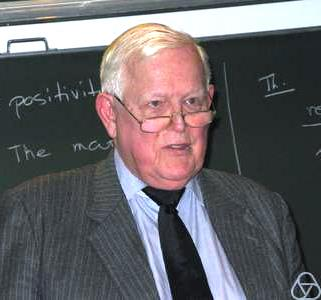
\includegraphics[scale=1]{Rudolf_Kalman.jpg} 
\caption{Rudolf E. Kalman}
\label{fig:kalman}
\end{figure}

\newpage

\tableofcontents

\newpage



\section{Introduzione}
Il filtro di Kalman è un osservatore ottimo dello stato per sistemi lineari in presenza di rumori gaussiani.

\newpage

\section{Cenni di teoria della probabilità}

Il filtro di Kalman è un algoritmo che mira alla ricostruzione dello stato interno di un sistema basandosi unicamente su una serie di misurazioni che, a causa di limiti costruttivi, sono soggette a rumore.

A causa della natura del problema, risulta necessario affrontare alcuni aspetti della teoria della probabilità, in particolare ci soffermeremo sul concetto di variabile aleatoria normale, o Gaussiana, con l'intento di fornire un modello matematico per gli errori di misura che siamo costretti ad affrontare.

\subsection{Variabili aleatorie o casuali.}

Una variabile casuale/aleatoria è una variabile che può assumere valori diversi in dipendenza da qualche fenomeno aleatorio.
In particolare diremo che una variabile casuale $X$ si dice continua se esiste una funzione $f(x)$ definita su tutto $\mathbb{R}$ : $P(X \in B) = \int_B f(x) dx$ dove la funzione $f$ si dice \textit{densità di probabilità} della variabile casuale $X$.

L'integrale di tale funzione nel dominio di integrazione $B$ rappresenta pertanto la probabilità che la variabile aleatoria assuma valori appartenenti a $B$.

Le variabili casuali risultano essere un valido strumento matematico per la modellazione dei rumori.

Alle variabili casuali sono associati i concetti di media/valore atteso, di varianza e di covarianza.

\subsubsection{Valore atteso}

Nella teoria della probabilità il valore atteso di una variabile casuale $X$, è un numero indicato con $E[X]$ che formalizza l'idea di valore medio di un fenomeno aleatorio.
\begin{equation}
\ {\mathbb  {E}}[X]=\int _{{-\infty }}^{{\infty }}xf(x)dx
\end{equation}

\noindent  Si noti che l'operatore valore atteso è lineare:
\begin{equation}
E[aX + bY] = aE[X] + bE[Y]
\end{equation}




\subsubsection{Varianza}

La varianza di una variabile aleatoria è una funzione che fornisce una misura della variabilità dei valori assunti dalla variabile stessa; nello specifico, la misura di quanto essi si discostino dal valore atteso.

La varianza della variabile aleatoria $X$ è definita come il valore atteso del quadrato della variabile aleatoria centrata sulla propria media: $X - E[X]$ :
\begin{equation}
Var(X) = E[(X - E[X])^2]
\end{equation}

\subsubsection{Covarianza}

In statistica e in teoria della probabilità, la covarianza di due variabili aleatorie è un numero che fornisce una misura di quanto le due varino dipendentemente l'una dall'altra.

La covarianza di due variabili aleatorie $X$ e $Y$ è il valore atteso dei prodotti delle loro distanze dalla media: \begin{equation}
Cov(X,Y)= E [(X-E[X])(Y-E[Y])]
\end{equation}
Due variabili casuali si dicono \textit{incorrelate} se la loro covarianza è nulla.

La covarianza può essere considerata una generalizzazione della varianza 
\begin{equation}
Var(X) = Cov(X,X)
\end{equation}

\subsection{Variabili gaussiane e modellazione dei rumori.}

Le variabili gaussiane sono particolari variabili aleatorie caratterizzate da due parametri, $\mu$ e $\sigma^2$, e sono indicate tradizionalmente con: 
\begin{equation}
X \sim N(\mu ,\sigma^2)
\end{equation}
Sono caratterizzate dalla funzione densità di probabilità: 
\begin{equation}
f(x) = \frac{1}{\sqrt {2\pi\sigma^2}}e^{-\frac{(x-\mu)^2}{2\sigma^2}}
\end{equation}
Si può dimostrare che per le variabili gaussiane vale che: 
\begin{equation}
E[X]= \mu \qquad Var[X]= \sigma^2
\end{equation}

Come anticipato possiamo modellizzare i vettori di disturbo del sistema che consideriamo, attraverso l'utilizzo di variabili aleatorie gaussiane a media nulla e varianza $\sigma^2$, di dimensioni conformi a quelle del sistema considerato.

\newpage
\subsection{Vettori casuali}

Un vettore casuale è un vettore i cui elementi sono variabili casuali.

Risulta necessario estendere le definizioni date in precedenza per caratterizzare rumori che agiscono su sistemi non scalari.

\subsubsection{Valore atteso}

Si dice valore atteso del vettore casuale $x \in \mathbb{R}^n$ il vettore dei valori attesi delle variabili casuali che lo compongono: 
\begin{equation}
E[x] = \begin{pmatrix}
E[x_1] & E[x_2] & \dots & E[x_n]
\end{pmatrix}^T
\end{equation}
Si definisce \textit{valore quadratico medio} di $x$ come $E[x^T x]$.

\subsubsection{Matrice di covarianza}

Si definisce \textit{matrice di covarianza} del vettore casuale $x \in \mathbb{R}^n$ la matrice $n \times n$: \begin{equation}
 Cov(x, x) = E[(x-E[x])(x-E[x])^T]
\end{equation}
Per come è definita, la matrice di covarianza è una matrice simmetrica semidefinita positiva i cui elementi $\sigma^2_{ij}$ sono le covarianze tra gli elementi $x_i$ e $x_j$ del vettore $x$.

A sua volta si definisce la matrice di \textit{cross-covarianza} tra due vettori casuali $x$ e $y$, la matrice
\begin{equation}
 Cov(x, y) = E[(x-E[x])(y-E[y])^T]
\end{equation}
Due vettori $x$ e $y$ si dicono \textit{incorrelati} se $Cov(x,y) = 0$.
\newpage

\documentclass[12pt,a4paper]{article}
\usepackage[utf8]{inputenc}
\usepackage[italian]{babel}
\usepackage{amsmath}
\usepackage{amsfonts}
\usepackage{amssymb}

\newcommand*{\matr}{\mathbf}
\newcommand*{\vett}{\mathbf}

\title{Automatica}

\begin{document}

\section{Automatica}
\subsection{Sistemi dinamici a tempo discreto}

Un sistema dinamico a tempo discreto è il modello matematico di un oggetto che interagisce con l’ambiente circostante attraverso canali di ingresso e di uscita che sono rappresentati attraverso vettori, $\vett{u}$ e $\vett{y}$, di variabili dipendenti dal tempo. La differenza principale dai sistemi a tempo continuo è che in questo caso il tempo è rappresentato come una variabile intera $k$.

Si avrà pertanto che per ogni istante di tempo $k$ il sistema riceverà dei segnali in ingresso e risponderà con dei segnali in uscita.

Il vettore $\vett{u} \in \mathbb{R}^m$ rappresenta i segnali che l’oggetto riceve dall’esterno mentre il vettore $\vett{u} \in \mathbb{R}^p$ rappresenta i segnali che l’oggetto dà in uscita.

In generale il comportamento del sistema non dipende esclusivamente da questi due vettori, ovvero non vi è un legame diretto tra ingresso e uscita: infatti il sistema ha uno stato interno che evolve in funzione degli ingressi e degli stati precedenti. In particolare lo stato di un sistema può essere a sua volta rappresentato da un vettore $\vett{x} \in \mathbb{R}^n$.

Il modello del sistema è pertanto costituito da equazioni che descrivono l’evoluzione dello stato del sistema in funzione dell’ingresso, dello stato e del tempo e esprimono la relazione d'uscita:
\begin{align*}
\vett{x}(k+1) &= \vett{f}(\vett{x}(k),\vett{u}(k),k) \\
\vett{y}(k) &= \vett{g}(\vett{x}(k),\vett{u}(k),k)
\end{align*}
dove $\vett{f}$ e $\vett{g}$ sono opportune funzioni vettoriali.

\subsection{Sistemi lineari stocastici}
Consideriamo una particolare tipologia di sistemi, quelli lineari strettamente propri, in cui le funzioni $\vett{f}$ e $\vett{g}$ sono appunto funzioni lineari e l’uscita non dipende esplicitamente dall’ingresso. In questo caso le equazioni si possono genericamente scrivere come:
\begin{align*}
\vett{x}(k+1) &= \matr{A}(k)\vett{x}(k) + \matr{B}(k)\vett{u}(k) \\
\vett{y}(k) &= \matr{C}(k)\vett{x}(k)
\end{align*}
dove $\matr{A},\matr{B},\matr{C}$ sono matrici di coefficienti variabili nel tempo.

Tuttavia tali modelli sono approssimazioni ideali che possono essere valide in alcuni contesti, mentre in altri è necessario tener conto delle incertezze e delle imprecisioni che si hanno nella misura dei segnali di ingresso e di uscita del sistema.

Tali incertezze possono essere modellizzate come vettori casuali:
\begin{align*}
\vett{x}(k+1) &= \matr{A}(k)\vett{x}(k) + \matr{B}(k)\vett{u}(k) + \vett{v}(k) \\
\vett{y}(k) &= \matr{C}(k)\vett{x}(k) + \vett{w}(k)
\end{align*}
In particolare si possono fare alcune ipotesi su tali variabili casuali:

\end{document}

\section{Osservatore ottimo}
Nella teoria del controllo, l'osservatore è un sistema dinamico che ha lo scopo di stimare lo stato di un altro sistema. L'osservatore è utile in quanto la conoscenza dell'evoluzione dello stato di un processo permette di risolvere problemi come la stabilizzazione e il controllo.

Nel caso di sistema lineare, l'osservatore può essere progettato come una copia del processo (del quale deve essere pertanto noto il modello) con l'aggiunta di un termine correttivo proporzionale alla differenza tra le uscite del processo e dell'osservatore. 

Tale osservatore prende il nome di \textit{Osservatore di Luenberger} ed ha la seguente espressione:
\begin{equation}
\label{obsv}
\hat{x}_{k+1}=A_k\hat{x}_k+B_ku_k+K_k(y_k-C\hat{x}_k)
\end{equation}

Si considera il sistema lineare con disturbi di processo e misura \eqref{rumlinsys},
con stato iniziale $x(k_0)=x_0$ e con ingresso $u_k$ misurabile per ogni $k \geq k_0$.

Per valutare la precisione dell'osservatore si definisce l'errore di stima, \\ $e_k \triangleq x_k-\hat{x}_k$, il quale è regolato da un'equazione dinamica che si può ottenere valutando tale espressione per $k=k+1$ e sostituendo sfruttando le equazioni \eqref{rumlinsys1} e \eqref{obsv}:
\begin{equation}
\label{errore}
\begin{split}
e_{k+1}&=A_kx_k+B_ku_k+W_kw_k-[A_k\hat{x}_k+B_ku_k+K_k(y_k-C\hat{x}_k)] = \\
&=(A_k-K_kC_k)e_k+W_kw_k-K_kv_k
\end{split}
\end{equation}
%Osserviamo che il valore atteso dell'errore è un sistema autonomo:
%\begin{equation}
%\bar{e}_{k+1}=E[e_{k+1}]=(A_k-K_kC_k)\bar{e}_k+ E[W_kw_k] - E[K_kv_k]=(A_k-K_kC_k)\bar{e}_k
%\end{equation}
Osserviamo che l'errore è a sua volta un sistema stocastico, dato che la sua espressione dipende dai termini $v_k$ e $w_k$, pertanto ne definiamo la matrice di covarianza all'istante $k+1$:
\begin{equation}
\label{matrcov}
P_{k+1}=E[e_{k+1}e_{k+1}^T]
\end{equation}
Tale matrice rappresenta l'\textit{errore quadratico medio} di stima all'istante $k+1$.

Per procedere con l'analisi ricordiamo le ipotesi \eqref{inizioipotesistatistiche}-\eqref{fineipotesistatistiche} fatte sui termini stocastici presenti nelle equazioni del sistema.

\section{Ottimizzazione}
L'obiettivo che ci si prefigge è quello di determinare la matrice $\matr{L}_k$ tale che la stima fornita dall'osservatore sia il più attendibile possibile.
In particolare si vuole minimizzare l'errore quadratico medio di stima:
\[E[\vett{e}_k^T\vett{e}_k]=tr(\matr{P}_k)\]
Tale problema prende il nome di \textit{problema dell'osservatore ottimo}.
Se la matrice $\matr{R}_k$ è definita positiva $ \forall k \geq 0$ il problema si dice\textit{non singolare }.
Si dimostra \citep{kalmanbucy} che la soluzione del problema non singolare dell'osservatore ottimo è costituita da:
\[\matr{L}_k = \matr{P}_k\matr{C}_k^T(\matr{C}_k\matr{P}_k\matr{C}_k^T + \matr{R}_k)^{-1}\]
dove $\matr{P}_k$ è la soluzione dell'equazione di Riccati scritta nella forma:
\[\matr{P}_{k+1}=-\matr{A}_k\matr{P}_k\matr{C}_k^T[\matr{R}_k+\matr{C}_k\matr{P}_k\matr{C}_k^T]^{-1}\matr{C}_k\matr{P}_k\matr{A}_k^T+\matr{A}_k\matr{P}_k\matr{A}_k^T+\matr{Q}_k\]
scegliendo come stima iniziale $\vett{\hat{x}}_0=\vett{\bar{x}}_0$.

Il dispositivo così ottenuto è detto osservatore ottimo a tempo discreto; esso viene frequentemente indicato anche come\textit{filtro di Kalman}.

La matrice $\matr{L}_k$ è detta matrice di guadagno del filtro.   


\section{Equazioni del filtro}

Il filtro di Kalman stima lo stato del processo in certi istanti di tempo e quindi realizza un feedback sulla base delle misure (rumorose).

Le equazioni del filtro di Kalman appartengono a due gruppi:
predizione dello stato e aggiornamento basato sulle misure.

Le equazioni di predizione dello stato proiettano in avanti lo stato corrente e la covarianza dell’errore di stima al fine di ottenere una stima a priori per il successivo istante temporale.
mentre le equazioni di aggiornamento dello stato realizzano il meccanismo in retroazione, cioè incorporano le nuove misure nella stima a priori per ottenere una stima a posteriori migliorata.

\begin{itemize}
\item[\textbf{Predizione:}]le equazioni proiettano lo stato e la covarianza dell’errore di stima in avanti dall’istante temporale $k-1$ all’istante $k$ 
\begin{align*}
\vett{\hat{x}}_k^- &= \matr{A}_k\vett{\hat{x}}_{k-1} + \matr{B}_k\vett{u}_k \\
\matr{P}_k^- &= \matr{A}_k\matr{P}_{k-1}\matr{A}_k^T + \matr{Q}_k
\end{align*}

\item[\textbf{Aggiornamento:}] prima viene calcolata la matrice dei guadagni di Kalman $L_k$, quindi le misure $y_k$ sono usate per generare una stima dello stato a posteriori. Alla fine, viene calcolata una stima a posteriori della covarianza dell’errore:
\begin{align*}
\matr{L}_k &= \matr{P}_k^-\matr{C}_k^T(\matr{C}_k\matr{P}_k^-\matr{C}_k^T + \matr{R}_k)^{-1}\\
\vett{\hat{x}}_k &= \vett{\hat{x}}_k^- + \matr{L}_k(\vett{y}_k - \matr{C}_k\vett{\hat{x}}_k^-)\\
\matr{P}_k &= (\matr{I} - \matr{L}_k\matr{C}_k)\matr{P}_k^-
\end{align*}

\end{itemize}
\newpage

\section{Documentazione software matlab}
In questo paragrafo viene descritta l'implimentazione del filtro di Kalman come sistema dinamico ed il task implementato dal nostro gruppo in ambiente di programmazione matlab.
\subsection{sistema.m}
Matlab presenta già una sua implementazione dei modelli dinamici ma in questo frangente si è preferita una sua nuova implementazione che includesse anche le matrici di covarianza degli errori di processo e di misura in modo da adattare più facilmente il problema alle nostre esigenze.\\
In particolare nel file \textit{sistema.m} viene implementata la \textbf{classe} dei sistemi dinamici che necessitiamo.\\
\subsubsection{Proprietà}
Le proprietà di cui dispone un oggetto di questo tipo sono :
\begin{lstlisting}[frame=single]
properties (Access = protected) % private, non modificabili.
	A,B,C,D,Q,R,x;	% A,B,C,D matrici del sistema
		% Q matrice di covarianza del rumore di processo
		% R matrice di covarianza del rumore di misura
	n,m,p;	% dimensioni rispettivamente di stato, ingresso e uscita
	xold;	% vettore degli stati vecchi (per plot)
	u;	% ULTIMO ingresso ricevuto
end
\end{lstlisting}

I metodi che implementa riguardano il costruttore dell'oggetto, l'evoluzione del suo stato interno e la lettura dell'uscita del sistema.\\
\newpage
\subsubsection{Costruttore}
La creazione dell'oggetto \textit{sistema} avviene tramite l'inizializzazione delle proprietà dell'oggetto in questione :
\begin{lstlisting}[frame=single]
function obj = sistema(A,B,C,D,Q,R,x0)
\end{lstlisting}
Al costruttore vanno passate tutte le matrici relative al caso preso in analisi (comprese le covarianze) ed il suo stato iniziale.\\
Al suo interno vengono effettuati svariati controlli sulle dimensioni delli matrici (e non solo) per far si che queste ultime rispettino le seguenti proprietà :
\begin{itemize}
\item A deve essere quadrata (dimensione nxn);
\item B deve avere n righe (dimensione nxm);
\item C deve avere n colonne (dimensione pxn);
\item D deve essere di dimensione pxm;
\item Q deve essere quadrata, di ordine m e definita positiva;
\item R deve essere quadrata, di ordine p e semidefinita positiva;
\item x0 vettore riga/colonna di dimensione n.
\end{itemize}

\subsubsection{Evoluzione dello stato}
In matlab nei metodi delle classi che utilizzano le proprietà delle stesse, risulta necessario passare come argomento l'oggetto corrente. Questo è possibile attraverso la parola chiave \textit{obj}.
\begin{lstlisting}[frame=single]
function update(obj, u) % aggiorna lo stato del sistema 
    if (nargin<2)
	u = zeros(obj.m,1);  % se u viene omesso si considera nullo
    end
    obj.u=u;            
    obj.xold(:,end+1)=obj.x;  % salva il vecchio stato
    xn=obj.A*obj.x + obj.B*obj.u + obj.B*mvnrnd(zeros(obj.m1),obj.Q)'; % calcola il nuovo stato x(t) = Ax(t-1) + Bu + v : v = rumore di processo
    obj.x = xn;	% aggiorna lo stato con quello nuovo            
end
\end{lstlisting}
La funzione accetta come parametro esterno l'ingresso dato al sistema.\\
Esso può essere omesso, in tal caso viene considerato nullo.\\
All'interno del metodo vengono inoltre aggiornate le variabili di stato del sistema.\\
Implementa l'equazione di stato $x(t+1)=Ax(t)+Bu(t)+v$
\newpage
\subsubsection{Letture}
Aggiornato lo stato interno del sistema è ovviamente possibile leggerne la risposta. Questo avviene tramite il metodo \textit{leggiUscita} che implementa l'equazione $y(t) = Cx(t)+Du(t)+w$ .\\
Il metodo non necessita di ulteriori argomenti in ingresso:

\begin{lstlisting}[frame=single]
function y = leggiUscita(obj) % restituisce in output l'uscita del sistema 
\end{lstlisting}

In più è stata implementata il metodo per la lettura dello stato interno in quanto l'accesso diretto alle proprietà del sistema è, per ragioni di sicurezza, privato all'oggetto stesso (consentito unicamente ad esso).
\begin{lstlisting}[frame=single]
function esc = leggiStato(obj) % get dello stato per plot.
\end{lstlisting}

\newpage

\subsection{kalmanfilter.m}
La classe klamanfilter è stata pensata come un estensione di un sistema dinamico (in particolare del sistema dinamico da osservare) con in più le matrici di guadagno caratteristiche.\\
Questo è implementabile attraverso il concetto di ereditarietà delle classi, infatti kalmanfilter eredita proprietà e metodi di sistema:
\begin{lstlisting}[frame=single]
classdef kalmanfilter < sistema 
\end{lstlisting}
\subsubsection{Proprietà}
Oltre alle proprietà caratteristiche dei sistemi dinamici, vengono introdotte le matrici di guadagno e di covarianza dello stato :
\begin{lstlisting}[frame=single]
properties (Access = protected)
	P,K; %rispettivamente covarianza stato e guadagno
	vecchieK;
end
\end{lstlisting}
\subsubsection{Costruttore}
Come in \textit{sistema.m} la classe \textit{kalmanfilter} accetta come argomenti in ingresso le matrici relative al sistema dinamico da osservare (così da non dover costruire prima un oggetto di tipo sistema) ed il suo stato iniziale ed in più, opzionalmente, una stima  iniziale della covarianza dello stato (P0). Se non fornita come stima iniziale viene considerata la matrice identità di ordine n:
\begin{lstlisting}[frame=single]
function obj = kalmanfilter(A, B, C, D, Q, R, x0, P0)
\end{lstlisting}

All'interno del costruttore viene chiamato il costruttore della superclasse (sistema) al fine di inizializzare le variabili relative ad esse nell'oggetto \textit{kalmanfilter} :
\begin{lstlisting}[frame=single]
	obj@sistema(A, B, C, D, Q, R, x0);
\end{lstlisting}

\subsubsection{Evoluzione}
Come per la superclasse corrispondente, la classe \textit{kalmanfilter} non avrà il metodo ereditato che calcolerà l'evoluzione del sistema da osservare ma un overload di essa in quanto necessita di un metodo che implementi le equazioni di predizione, guadagno e correzione descritte nei paragrafi precedenti.\\
Questo avviene attraverso il metodo :
\begin{lstlisting}[frame=single]
function update(obj, u, y) % stima lo stato
\end{lstlisting}
i cui parametri d'ingresso sono rispettivamente l'ingresso e l'uscita del sistema da osservare al tempo $t$.\\
Anche quì si necessitano dei metodi di GET delle variabili interne all'oggetto.
\newpage

\subsection{Main task : filtraggio.m}
Il task che ci siamo prefissati di raggiungere è quello di ricostruire un segnale disturbato da rumore bianco. Questa applicazione risulta molto frequente in ambito ingegneristico in quanto anche i migliori trasduttori, per limiti costruttivi, presentano delle variazioni nelle misure seppur piccole.\\
Oltre a questo i trasduttori migliori presentano un costo elevato, per cui si può pensare di risparmiare sulla sensoristica applicando, alle misure più rumorose di un eventuale trasduttore economico, il filtro di Kalan così da ottenere dei valori affidabili a prezzi più accessibili.
\\
\begin{wrapfigure}{r}{1in}
\centering
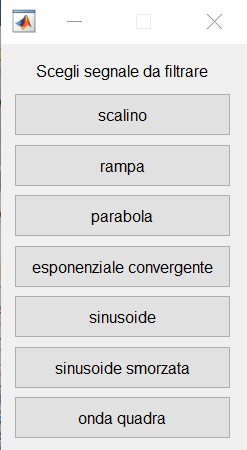
\includegraphics[scale=.7]{immaginiMain/mainfilterPOSS.png} 
\end{wrapfigure}
Una volta cliccato il pulsante \textit{Run} di matlab la prima schermata permette la scelta del segnale da filtrare.
A destra il layout di tale schermata con tutte le possibili scelte cliccabili.\\
Cliccando uno dei segnali il programma provvederà alla creazione del sistema relativo alla generazione di tale segnale.
\begin{lstlisting}[frame=single]
sys = ss(A,B,C,D);
sysd = c2d(sys,dt);
[Ad,Bd,Cd,Dd] = ssdata(sysd);
\end{lstlisting}
Successivamente viene assegnata la matrice di covarianza del rumore di processo :
\begin{lstlisting}[frame=single]
Q = 1e-5;
\end{lstlisting}
A questo punto si procede alla generazione dell'oggetto della classe kalmanfilter, che verrà utilizzato per la stima e il filtraggio del segnale, utilizzando le matrici relative alla discretizzazione del modello precedente e lo stato 0 come stato iniziale.
\begin{lstlisting}[frame=single]
k=kalmanfilter(Ad,Bd,Cd,Dd,Q,R,x0,P0);
\end{lstlisting}

A questo punto il programma procede con il calcolo dell'evoluzione dello stato e con il plottaggio e l'animazione della stima effettuata dal filtro, il tempo dell'animazione, e la variazione delle matrici di  covarianza dello stato e del guadagno.\\
Di seguito viene riportato un esempio del filtraggio di uno scalino affetto da rumore :


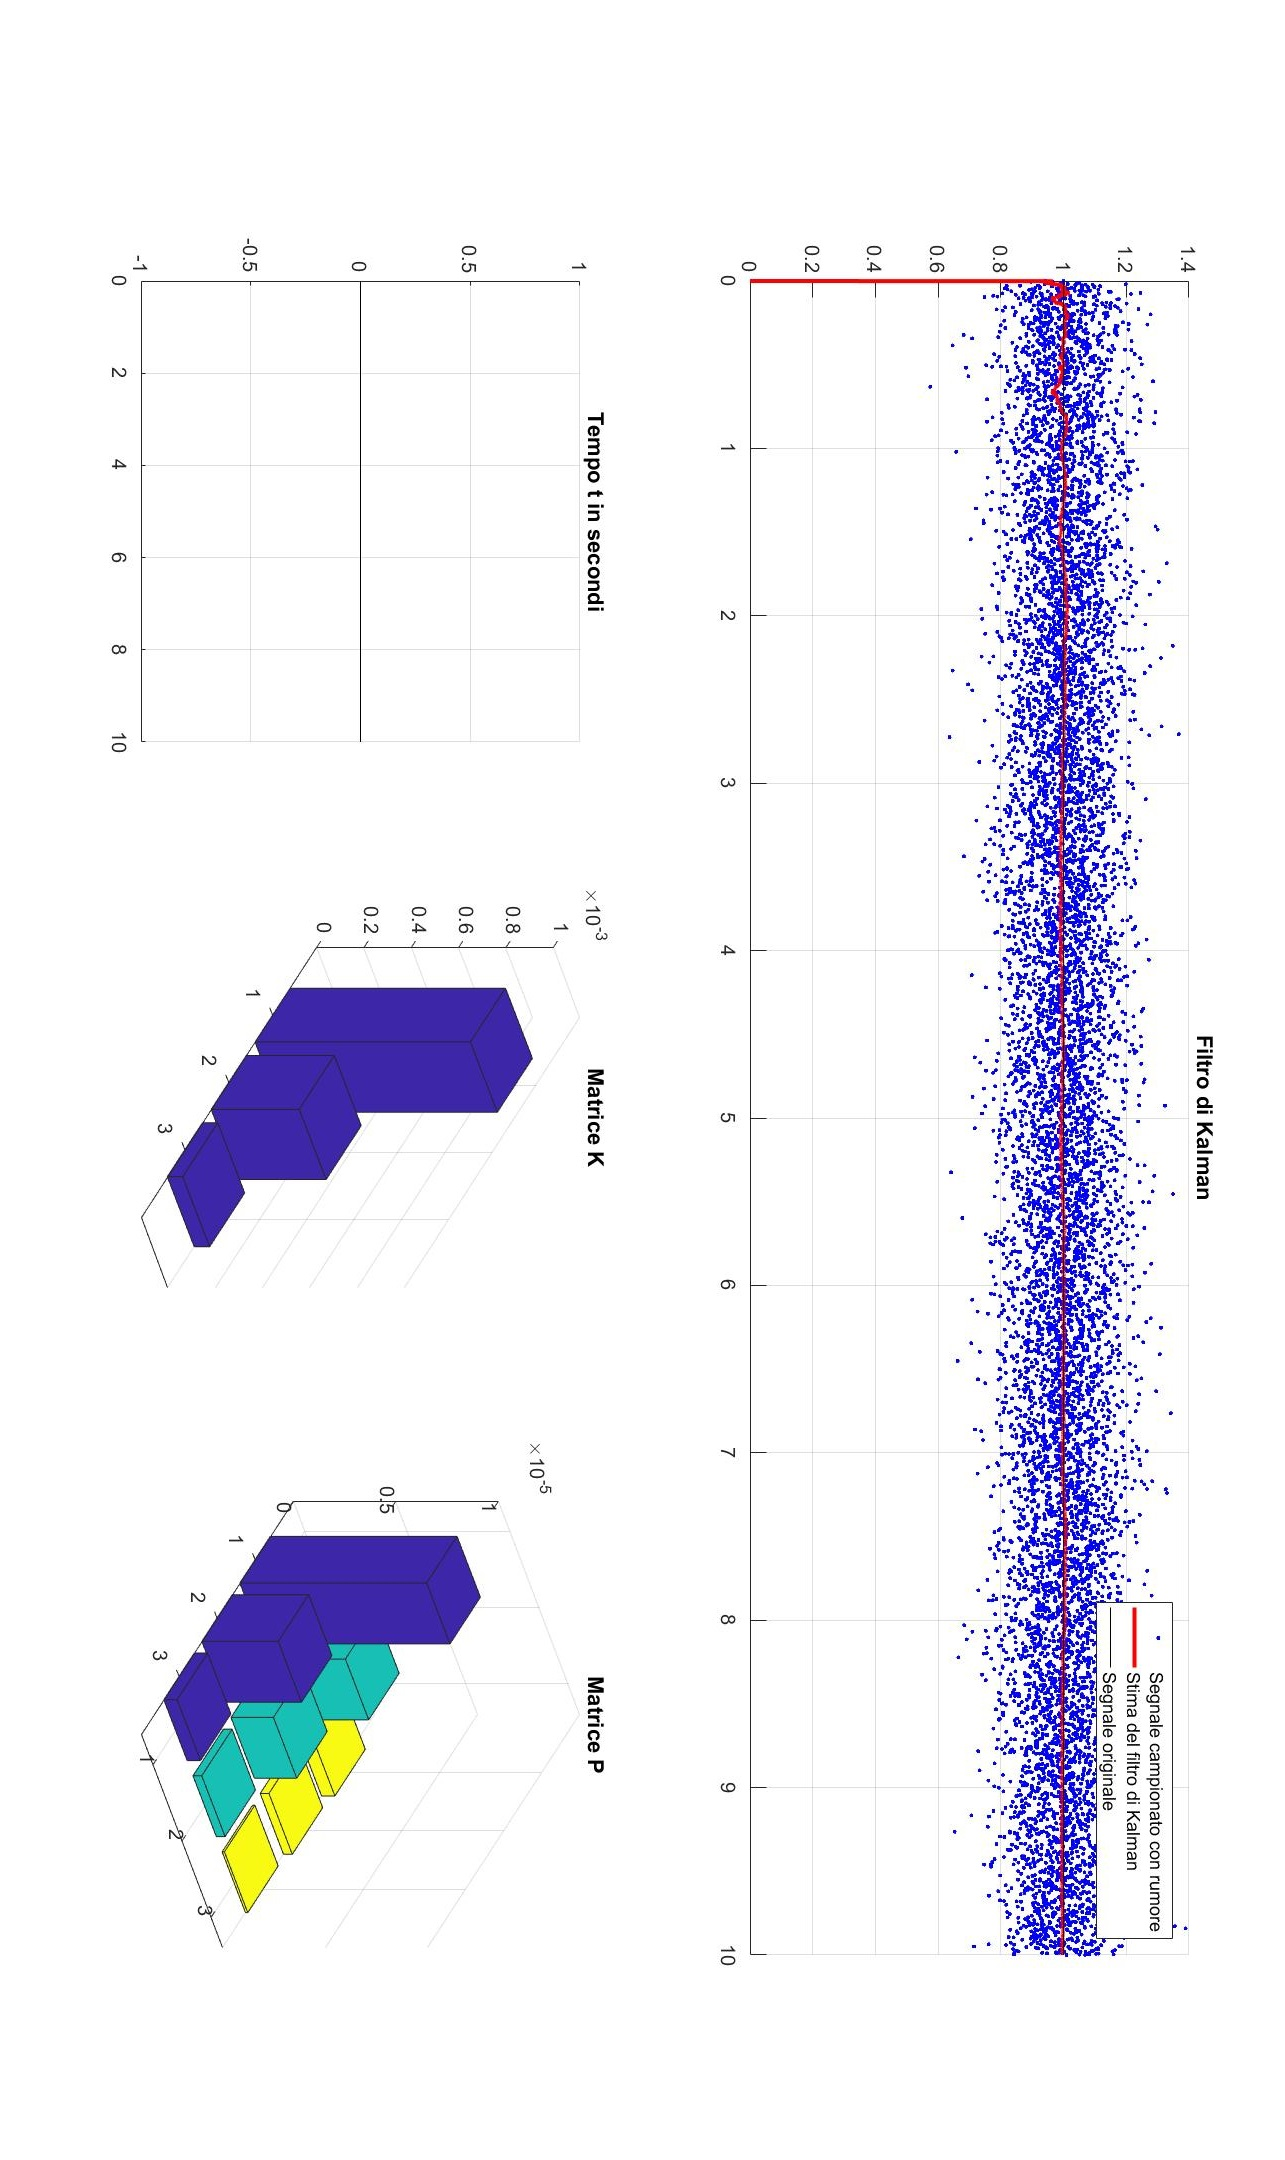
\includegraphics[scale=.5]{immaginiMain/esempio.jpg} 




\newpage

\section{Conclusione}
"A nonlinear differential equation of the Riccati type is derived for the covariance matrix of the optimal filtering error. The solution of this 'variance equation' completely specifies the optimal filter for either finite or infinite smoothing intervals and stationary or non-stationary statistics.
The variance equation is closely related to the Hamiltonian (canonical) differential equations of the calculus of variations. Analytic solutions are available in some cases. The significance of the variance equation is illustrated by examples which duplicate, simplify, or extend earlier results in this field.
The duality principle relating stochastic estimation and deterministic control problems plays an important role in the proof of theoretical results. In several examples, the estimation problem and its dual are discussed side-by-side.
Properties of the variance equation are of great interest in the theory of adaptive systems. Some aspects of this are considered briefly."\citep{kalmanbucy}
\newpage
\bibliographystyle{plain}
\bibliography{references}
\end{document}
